\documentclass[10pt,a4paper,abstract=on]{scrartcl} %scrartcl from KOMA-script uses sans headers and looks less latexy than article
\usepackage[doublespacing]{setspace}
%\usepackage[capposition=top]{floatrow} %for notes under pics
%\usepackage[nomarkers]{endfloat}
\usepackage{natbib}
\usepackage[utf8]{inputenc}
%\usepackage{amsmath}
%\usepackage{amsfonts}
%\usepackage{amssymb}
\usepackage[left=2.5cm,right=2.5cm,top=3cm,bottom=3cm]{geometry}
\usepackage[pdftex, hidelinks]{hyperref} %disable if using float package
\usepackage{graphicx}
\usepackage{booktabs}
\usepackage[blocks]{authblk} %for affil
\usepackage{url}
\usepackage{tabularx}
%\usepackage{float} %allows the H positioning specifier; conflicts with hyperref
\usepackage{csvsimple}
\usepackage[nomessages]{fp}
\usepackage{xcolor}
\usepackage{enumitem}
\setlist{noitemsep} % \setlist{nosep} to reove separation around lists as well
\usepackage[flushleft]{threeparttable}
\usepackage{dcolumn}
\usepackage{lineno, blindtext}
\usepackage{pdflscape}

%citation cheat sheet:
	%\ cite{key}				Jones et al. (1990)
	% \citet{key1,key2}			Jones et al. (1990); Ladze (1986)
	% \citet{key}				Jones et al. (1990)
	% \citet*{key}				Jones, Baker, and Smith (1990)
	% \citep{key}				(Jones et al. 1990)
	% \citep{key1,key2}			(Jones et al. 1990; Ladze 1986)
	% \citep*{key}				(Jones, Baker, and Smith 1990)
	% \citep[p.~99]{key}		(Jones et al., 1990, p. 99)
	% \citep[e.g.][]{key}		(e.g. Jones et al., 1990)
	% \citep[e.g.][p.~99]{key}	(e.g. Jones et al., 1990, p. 99)
	% \citeauthor{key}			Jones et al.
	% \citeauthor*{key}			Jones, Baker, and Smith
	% \citeyear{key}			1990
	% \citealt{key} 			Jones et al. 1990


\newcommand{\figureloc}{C:/Users/Koen/Dropbox/PhD/Papers/CongoGBV/Figures}
\newcommand{\tableloc}{C:/Users/Koen/Dropbox/PhD/Papers/CongoGBV/Tables}
\newcommand{\bibloc}{C:/Users/Koen/Dropbox/Literatuur/Mendeley/Bibtex/CongoGBV}



%create table for mean differences
\csvstyle{meandifftable}{tabular=lccccc,table head= \toprule Variable & N &Control & Treatment & Diff & St. Err. \\\toprule,late after line=\\,table foot=\bottomrule}

\newcommand{\meandifftab}[1]{
	\begin{threeparttable}
	\csvreader[meandifftable]{#1}%
	{n0 = \na, n1= \nb, label0 = \laba, label1 = \labb, varlabel=\var,meancontrol0 = \mca, meantreat0 = \mta ,stardiff0=\diffa, sediff0=\sea, meancontrol1 = \mcb, meantreat1 = \mtb , stardiff1=\diffb, sediff1=\seb, stardd = \dd, sedd=\sedd}%
	{%
	\var  	& 		& 		& 		& 		 &		\\ %
	\quad \laba 		& \na	& \mca 	& \mta 	& \diffa & \sea	\\%
	\quad \labb 		& \nb	& \mcb 	& \mtb 	& \diffb & \seb	\\%
	\quad Diff in Diff 	& 		&		&		& \dd 	 & \sedd
	}%
	\begin{tablenotes}
	\small
	 \item Robust Standard errors reported.
	 \item * p $<$ 0.1, **, p $<$ 0.05, *** p $<$ 0.01
	\end{tablenotes}
	\end{threeparttable}
}


\begin{document}

\author{Koen Leuveld}

\affil{Development Economics Group, Wageningen University \\
koen.leuveld@wur.nl}



\title{Sexual Violence, conflict, intra-household relations and gender norms}
\subtitle{Exploratory evidence from a list experiment in Eastern DR Congo} %needs scrartcl

\maketitle

\begin{center}
\textcolor{red}{\Large EARLY DRAFT}
\end{center}

\begin{abstract}
%\section*{}
%\paragraph{Abstract}
The high incidence rates of Sexual and Gender-based Violence in the Democratic Republic of the Congo present a large human rights problem. While this high incidence has often been associated with the violent conflict in the country, much is unclear about the drivers of SGBV, as accurate data on the subject is difficult to collect. In order to obtain reliable data on this incidence, and to avoid social desirability bias, I conducted a list experiment. I combine the data from this list experiment with rich data on respondents' households, including conflict history, female bargaining position and social norms. 

I find mixed evidence for the correlation between victimization of SGBV and victimization of the conflict: victimization in the past twelve month is not explained by recent conflict, but is associated with historic conflict. A possibly explanation for this is that conflict negatively affects norms and the position of women in society, and in this way has an indirect effect on SGBV. I do find a strong correlation between victimization of SGBV and the intra-household bargaining position of women: the result from a bargaining game, and the pre-marriage relative status of the wife and husband. As for gender norms, I find no evidence of correlation between more empowered norms, and lower incidence of SGBV.
\end{abstract}

\linenumbers
%literature to add somewhere:
%\cite{Saile2013} investigate the correlates of Intimate Partner Violence for a sample of conflict-exposed women in Northern Uganda. They find that while the level of conflict exposure predicts physical violence, sexual violence is more associated with the level of childhood familial violence. This link between current and past experiences of violence suggests that the effect of conflict on violence is deeper than just the direct effect. People traumatized during the conflict (either because they were victims or perpetrators) are more likely to be victimized later on. CHECK OOK NOG DE REFERENTIES VOOR EEN DIEPERE ONDERBOUWING VAN DIT PUNT.

%\cite{Muller2019} investigate the link between the conflict in Gaza and Domestic Violence. They find that exposure to conflict increases the incidence of DV. A woman's bargaining position decreases the incidence. IN DE LIT LIJST MEER ARTIKELEN OVER IPV <-> VIOLENCE

%\cite{Boesten2018}: collection of papers with some qualitative blabla. Could be worthwhile.


%%%%%%%%%%%%%%%%%%%%%%%%%%
\section*{Introduction}
%%%%%%%%%%%%%%%%%%%%%%%%%
%Hook
The high incidence of Sexual and Gender Based Violence (SGBV) in the Congo has been a prominent area of attention for the international development community over the past decades. Often, this high incidence of SGBV has been linked to the various violent conflicts the country has seen since the 1990s. In international policy circles, attention for the link between conflict and SGBV increased at the end of 1990s, when rape was used strategically by armed actors during armed conflicts in Rwanda and Bosnia  \citep{Kirby2015}. This issue of conflict-related SGBV in Congo in particular has been on the agenda since 2002 when the NGO Human Rights Watch published a report on the topic \citep{HRW2002}. Since then, the issue has received attention by the UN, governments, NGOs and even celebrities \citep{Baaz2013}. This attention is understandable, given the high psychological, social and economic costs of SGBV, even outside conflict settings \citep{Post2002,Peterson2018}. Consequently, Congo has nearly become synonymous with rape, even called the ``rape capital of the world'' by the UN's Special Representative on Sexual Violence in Conflict, Margot Wallstrom. Tremendous international efforts have been made to implement or support projects to assist the victims of SGBV. The 2018 Nobel Peace prize was awarded to Dr. Denis Mukwege, for his work on victims of SGBV at Bukavu's Panzi Hospital.
 
%research question
%make sure this flows better.
To adequately address this issue, data on the victims of SGBV is of crucial importance. In this paper, I explore the characteristics of the victims SGBV to uncover the dynamics and potential drivers of SGBV.

%Antecedents
While estimates for the incidence of SGBV in DR Congo vary, they are invariably high: ranging from 15\% to 40\% \citep{Johnson2010,Peterman2011}. The variation in these estimates is likely caused by different ways of collecting data (e.g. population-level vs. clinic-based surveys), under-reporting by victims, and the difficulties in obtaining good quality data in Congo. The conflict that has persisted in the country for the past decades has been frequently cited as the most important driver of SGBV. This is particularly true for policy circles, where the framing of SGBV in Congo as ``weapon of war'' is popular \citep{Baaz2013,Kirby2015}. There is empirical evidence to support this notion. \cite{Johnson2010} carried out a large-scale survey in Eastern DRC to investigate incidence and perpetrators of SGBV, and found that the majority of sexual violence reported by their respondents was conflict-related; of female victims of sexual violence, 74.3\% reported the perpetrators to be conflict-related. It is therefore not surprising that the topic of SGBV in Congo has often been analysed within the context of violent conflict \citep{Baaz2013}. Likewise, the aspect of the conflict that has received the most world-wide media attention has been SGBV \citep{Autesserre2012a}.  

This view of the central role of conflict in sexual violence in the DRC has come under increasing scrutiny. It has been argued that this focus on the relationship between sexual violence and conflict has been counter-productive, as it has distracted attention from other pressing problems the DRC faces \citep{Autesserre2012a, Hilhorst2018,Porter2019}. Moreover, it risks missing the civilian perpetrators of SGBV. There is empirical evidence for this position too. Based on DHS data, \cite{Peterman2011} find that rates of Sexual Intimate Partner Violence (IPV) are higher than rates of other forms of Sexual Violence in Congo. 

This increased focus on IPV, rather than conflict, shifts attention from conflict to two other drivers of SGBV: female empowerment and cultural norms. Here, I use the term Female empowerment to refer to the bargaining position of individual women in their household. The effect of improving this bargaining position on SGBV is ambiguous \citep{Eswaran2011}. One the one hand, a woman's welfare may depend on her bargaining position, as determined by outside options. Women with more income, and better prospects in case of a divorce would thus face less risk of IPV. On the other hand, as a response to her increased empowerment, a  woman's partner may use IPV as an instrument to assert power. The empirical record reflects this ambiguity. \cite{Bhattacharya} find that increase in employment, and the increasing of status of a woman within the household reduces violence. Similarly, \cite{Hidrobo2016} find that cash transfers to women, decrease the risk of violence. However, when specifically looking at sexual IPV in the Dominican Republic, \cite{Bueno2017} find that an increase in women's (economic) empowerment led to an increase in IPV. The link between IPV and women's intra-household bargaining position may be moderated by local customs, and depend on exactly the type of IPV and the type of empowerment under consideration.

In addition to the empowerment, attitudes and customs are often cited as risk factors for SGBV. Increasing gender awareness, and improving cultural norms are a common policy recommendation when it comes to preventing SGBV \cite[e.g.][]{Quattrochi2019,Bueno2017}. \cite{Hilhorst2018} argue that the local NGO community in Eastern Congo is well aware of this, and uses the increased funds related to the massive attention generated by the ``weapon of war'' account of SGBV in Congo to fund projects to improve female empowerment in Congo and in this way prevent SGBV.  However, there is a long way to go, and women still hold a precarious position in Congolese society. For example, views that men have the right to physically abuse their wife if she is disobedient are broadly held \citep{Quattrochi2019}.

Conflict and the two drivers of IPV are not necessarily separate, as the effect of conflict on the incidence of SGBV can be direct and indirect. The direct mechanism is what caused the topic to be on the international agenda; the perpetration of SGBV by armed groups; potentially in a strategic manner \citep{Baaz2013,Kirby2015}. However, there is a more indirect effect as well: conlfict causes the breakdown of norms, which may have long-lasting effects. For example, \cite{Kelly2018} find that that IPV increased in districts that experienced conflict in Liberia, while \cite{Muller2019} find draw similar conclusions from data from the Gaza strip. \cite{Saile2013} investigate the correlates of IPV for a sample of conflict-exposed women in Northern Uganda. They find that while the level of conflict exposure predicts physical violence, sexual violence is more associated with the level of childhood familial violence. This link between current and past experiences of violence suggests that the effect of conflict on violence is deeper than just the direct effect. People traumatized during the conflict (either because they were victims or perpetrators) are more likely to be victimized later on. 


%Bouta, T., G. Frerks, and I. Bannon (2005) Gender, Conflict and Development. The World Bank, Washington, DC
%Tia Palermo and Amber Peterman, ‘Undercounting, overcounting and the longevity of flawed estimates: statistics on sexual violence in conflict’, Bulletin of the World Health Organization, no. 89, 2011, pp. 924–5;
A large problem underlying the analysis of drivers and dynamics of SGBV is the paucity of reliable data \citep{Palermo2011}. This is exacerbated by the fact that the empirical studies that do exist, contradict each other. While one study finds conflict-related perpetrators are responsible for the majority of cases of SGBV \citep{Johnson2010}, another finds intimate partners as the most common culprits \citep{Peterman2011}. \citet{Stark2017} provide a possible explanation for this discrepancy. In a study where 87 women and girls in South Kivu were interviewed using Audio Assisted Self-Interviews (ACASI) techniques,they find that 14\% of respondents reported having been victim of sexual coercion. Half of these were perpetrated by the respondents' husbands or boyfriends. Crucially, in complementary group discussions, respondents did not bring up intimate partners at all. This points at the difficulties of collecting accurate data about SGBV, and the importance of data collection methodologies. 

%Contribution
%I combine these three items into one research.
This paper contributes to the empirical evidence base on the incidence of SGBV in Eastern Congo by using a list experiment to obtain reliable estimates of the incidence of SGBV. List experiments remove the bias in answering sensitive question, by removing the possibility of the researcher (or anyone else) to view individual answers to the sensitive topic. However, group-level analysis is still possible, to provide estimates of correlates of SGBV. This data is obtained from surveys implemented as part of the evaluation of four development projects in South Kivu province. This household survey, including rich data on the household and outcomes from behavioural experiments, allows for a rich characterization of victims of SGBV.  Because such a characterization is lacking thus far, this data is useful in addressing and preventing SGBV. Moreover, while the potential drivers of SGBV mentioned above -- conflict, intra-household dynamics, and gender attitudes -- have been studies in isolation, this paper contributes by analysing these in one framework.
%perhaps note that tia finds no predictors for SGBV.

%Road Map
I find mixed evidence for the correlation between victimization of SGBV and victimization of the conflict: victimization in the past twelve month is not explained by recent conflict, but is associated with historic conflict. A possibly explanation for this is that conflict negatively affects norms and the position of women in society, and in this way has an indirect effect on SGBV. I do find a strong correlation between victimization of SGBV and the intra-household bargaining position of women: the result from a bargaining game, and the pre-marriage relative status of the wife and husband. As for gender norms, I find no evidence of correlation between more empowered norms, and lower incidence of SGBV. This early draft of the paper is structured as follows: first I describe the research setting and data. The subsequent section describes my empirical framework, which revolves around the use of a list experiment. I then present the correlates of SGBV that are considered in this paper, followed by a discussion of the results of the analyses. In the concluding remarks, I contextualize the findings and present policy implications.

%%%%%%%%%%%%%%%%%%%%%%%%%%%%%%%%
\section*{Background and Data}
%%%%%%%%%%%%%%%%%%%%%%%%%%%%%%%%
SAMPLE IS GEWIJZIGD: DE GETALLEN IN TEKST EN TABELLEN VERSCHILLEN HIER EN DAAR

\newcommand{\summstat}[2]{\csvreader[filter strcmp={\var}{#1}]{\tableloc/balance.csv}{var=\var,#2=\stat}{\stat}}

%command to retrieve summary statistics from balance.csv
%include map
%conflict in the study area
The present study is set in the territories of Fizi and Uvira, South Kivu province, in the east of the Congo bordering Burundi and Rwanda. The conflicts in the Congo were particularly intense in this area. After the Rwandan genocide in 1994, South Kivu housed many camps for Rwandan refugees. The presence of \textit{genocidaires} among these refugees was cause for Rwanda to invade Congo (then know as Zaire), putting the province on the front line of the conflict. Throughout this First Congo War (1996-1997), the Second Congo War (1998-2003) and the subsequent fragile peace, ethnic tensions have remained high throughout the area, resulting in frequent localized bursts of violence.

The Human Rights Watch report responsible for putting the topic of war-time SGBV in Congo on the international agenda identifies several areas of the study region as particularly hard-hit by both conflict and SGBV \citep{HRW2002}. Fizi in particular, is identified as a dangerous place for women during the war. These instances of abuse did not only happen during attacks on villages, but also during ambushes; women travelling to their farms, or to markets to buy or sell produce were at risk from armed groups. Uvira, in contrast, has suffered more to the ethnic violence following the 2003 peace agreements.

The main source of data for this study is a household survey that was undertaken in 2014 as the endline survey for the evaluation of Dutch development aid. This evaluation concerned projects ran by four NGOs in the territories of Kabare, Fizi and Uvira, and the commune of Bagira (which will be included with the territory of Kabare, since the selected communities in Kabare and Bagira are close together). The baseline for this evaluation was done in 2012. Half of the respondents were selected from communities that benefited from the projects, the other half were selected from similar households in non-intervention communities. These projects were about agriculture, women's rights and education. Overall, the beneficiaries of the projects vulnerable, mostly rural, households. In total data was collected in 73 communities. In each community, baseline data was collected on 15 households in 2012; however, due to attrition, 2014 data is available for an average of 12 households per community, for a total of 889 households. 

\begin{threeparttable}
	\caption{Dempographics for DHS data and sample}\label{tab:dhs_compare}
	\centering
	{
\def\sym#1{\ifmmode^{#1}\else\(^{#1}\)\fi}
\begin{tabular}{l*{4}{c}}
\hline\hline
                    &\multicolumn{1}{c}{DHS National}&\multicolumn{1}{c}{DHS South Kivu}&\multicolumn{1}{c}{Full Sample}&\multicolumn{1}{c}{Gender Module}\\
                    &        mean&        mean&        mean&        mean\\
\hline
Age of FR           &       31.83&       31.09&       40.58&       41.09\\
Household has a tin roof&        0.33&        0.60&        0.58&        0.61\\
FR completed primary education&        0.47&        0.29&        0.25&        0.25\\
FR completed secondary education&        0.10&        0.06&        0.02&        0.03\\
\hline\hline
\end{tabular}
}

	\begin{tablenotes}
	\small
	\item FR stands for Female respodent. For the DHS data, means are provided for female heads of household, or female spouses of household heads. Data source columns 1 \& 2: \citep{DHSCongoReport}
	\item
	\end{tablenotes}
	
\end{threeparttable}

The sampling procedure outlined here is thus unlikely to have produced a nationally (ore even provincially) representative sample. In Table \ref{tab:dhs_compare} a comparison across selected demographics between the full study sample (column 3), and the representative sample from the DHS Program (columns 1-2) is presented. Women in the study sample are older, and less likely to have finished school, than the provincial average in South Kivu.


\begin{table}[htb]
\centering
\caption{Gender module sample make up}
\label{tab:bargsample}
\begin{tabular}{l c c c c c}
\toprule
 & \multicolumn{5}{c}{Husband} \\
Wife&Consented&Refused&Absent&No Husband&Total \\
&No.&No.&No.&No.&No. \\
\hline
Consented&184&3&253&153&593 \\
Refused&0&0&0&1&1 \\
Absent&4&0&0&1&5 \\
No Wife&282&3&2&3&290 \\
Total&470&6&255&158&889 \\
\bottomrule
\end{tabular}
\end{table}

%kan ik misschien dat stukje "for convenience" aanpassen?
The survey contained a gender module that: (i) collected detailed information on gender attitudes; (ii) contained a list experiment designed to elicit the incidence of SGBV among female respondents; and (iii) contained a risk bargaining game. Where possible, this gender module was administered to both the head of the household and the spouse of the household head. In the vast majority of the cases, the husband is considered the head, but it was left open to the respondent to indicate the head. Table \ref{tab:bargsample} displays how the sample is built up. In total, there were 889 respondents to the survey. In 593 households, the female respondent (the wife of the household head or the single female head) consented to responding to the gender module. In 1 household, the female respondent refused; in 5, the female respondent was absent during the interview, and in 290 households the head of the household had no wife, and there was thus no female respondent. In 470 households, the male respondent (usually the household head) consented to the module, 6 refused, 255 male respondents were absent, and in 158 households the head of the household was an unmarried woman, meaning that there was no male respondent. For 184 households, we have both husband and wife responding to the module. Efforts to increase this number, by tracking down absent household heads, were constricted by the limited time field teams had in each community, due to the security situation at the time of field work.

%expand this section, maybe?
The selection of respondents to the gender module is unlikely to have been random. In column 4 of Table \ref{tab:dhs_compare} selected demographics for the Female Respondents to the gender module are presented. The respondents are slightly older than the full sample, and considerably older than the provincial average. They are slightly more likely to have completed secondary school than the full sample, but less likely than the provincial average. Table \ref{tab:sample_selection} presents results from logit models models to find correlations between household characteristics and participation in the gender module. The dependent columns of the columns are whether the wife, the husband and the couple participated in the gender module. There are some selection effects: households where a female respondent is present, are less likely to own livestock. On the contrary, households where the husband participated were more likely to own several types of livestock. This suggests that care must be taken when applying the findings from this study to the wider population.

\section*{Empirical Strategy}
%what are they?
%A qualitative analysis of disclosure patterns among women with sexual violence-related pregnancies in eastern democratic republic of congo
A major concern in collecting data on SGBV is reporting bias. Respondents are unlikely to be comfortable to truthfully answer questions about SGBV. What's worse, this unwillingness may be correlated to the identity of the perpetrators \citep{Stark2017}. Using answers to direct questions would thus lead to an underestimate of the incidence of SGBV, and biased estimates for the correlates of SGBV, due to the non-random nature of non-response. List experiments have gained popularity in recent years as a way to address this social desirability bias by not asking the sensitive question directly. Instead, respondents are presented with a list of issues and indicate the number of issues from the list they have faced. By adding the sensitive item to the list of issues for half of the respondents (randomly selected), estimates for incidence of the sensitive item can be obtained by comparing the mean number of issues faced in both groups (hence ``item count technique'' as an alternative name for list experiments). The advantage is thus that answers are guaranteed to be anonymous: the interviewer (or the data analyst) does not know the number of non-sensitive issues the respondent faces and so has no way of knowing the answer to sensitive item. This anonymity removes the need to hide the answer. 

%examples:
%\cite{Chuang2019} find that LEs weren't very precise.
%\cite{Peterman2018}
%add some more examples of things that have been studied using LEs.
\cite{Holbrook2010} review 48 studies using list experiments, and found that they are effective at decreasing social desirability bias. Comparing studies that use list experiments with studies that don't, they find that reporting rates of sensitive items are higher in studies using list experiments. It is therefore not surprising that this approach has been applied to a wide range of topics, such as sensitive political opinions \citep{Frye2017,Blair2014,Meng2017} and SGBV \citep{Bulte2019}. \cite{Bulte2019} is of particular interest to the current paper. They compare the results of direct questioning and list experiment to assess the incidence of IPV among beneficiaries of a program to boost female empowerment in Vietnam. They find that using direct questioning yields lower estimates of the incidence of IPV than direct questioning and argue that this is due to the social desirability bias in direct questioning. Moreover, they find the treatment effect of the project reverses its sign when using the list experiment. This underlines the potential of list experiments to address potential biases caused by reporting bias and direct questions.

%hoe ziet mijn implementatie er uit/
For the list experiment in this study, the female respondents were randomly divided into two groups. This was done by the electronic survey software (ODK), based on the randomly assigned ID codes. I follow \cite{Imai2011} in calling these groups Treatment and Control. The groups were told by the interviewer; ``I will read 4 (or 5) problems that women can experience. These can be sensitive problems. When you've experienced a problem in the last year, please drop one of the balls to the ground. I will not look at when you drop these balls, and only want to know the total number of balls at the end.'' The first group (Control) was presented with the following four control items:
\begin{itemize}
	\item Lack of food;
	\item Lack of money;
	\item Theft; and,
	\item Sterility. %sell dit, mensen kunnen hier moeite mee hebben. Is er een manier om te checken? zeker! check \cite{Chuang2019}!
\end{itemize}

Women in the second group (Treatment) were presented with the same four items, but a fifth item was added: Sexual Violence.  The four control items have been selected in such a way that it is unlikely women in the sample face none, or all, of the issues. This avoids ceiling or floor effects, where the interviewer knows the respondent's answer to the SGBV item if no issues are reported, or if all issues are reported. Not all the control items are non-sensitive, as the item ``sterility'' is a sensitive item. This was done to reduce respondent suspicion when one sensitive items is juxtaposed with a number of completely non-sensitive items (see \citet{Chuang2019} for a more detailed explanation). After all items were read, the interviewer asked the respondent to count the number of balls, and report the number. The questionnaire was field tested prior to field work to ensure that respondents understood these concepts. All interviewers were thoroughly trained in the protocols, and the electronic questionnaire was programmed in such a way to ensure compliance to the protocol.

A crucial assumption for the list experiment, is that the randomization ensures that Treatment and Control groups are identical. Table \ref{tab:balance} (Column 7) provides a comparison of the two groups within the sample. The treatment and control group are not perfectly balanced across some of the variables. As randomization was done at the time of data collection (based on randomly assigned ID codes). An F-test on the differences between treatment and control being jointly equal to zero fails to reject the null-hypothesis that they are equal (p=0.20). However, care should be taken in interpreting the differences in the variables with differences: results being closer to the women's choice, and the cash income of the household. 

%hoe doe ik de analyse, en interpreteer ik coefficienten etc.
While the indirect nature of list experiments prevents reporting bias, this does come at a cost of efficiency in statistical analysis. The incidence is easily computed by subtracting the mean of issues faced in the control group from the mean number of issues in the treatment group. This means that sample sizes have to be far larger for list experiments than for direct questions. 

In a regression framework, the incidence would be estimated as follows \cite{Holbrook2010}:

\begin{equation}
\label{eq:basic}
NumIssues_i = \beta_0 + \beta_1 Treatment_i + \epsilon_i
\end{equation}

Where \(NumIssues_i\) is the number of issues faced by respondent $i$, and \(Treatment_i\) is her treatment assignment. Coefficient \(\beta_1\) yields the estimate for the incidence. To find correlates of SGBV, equation \ref{eq:basic} can be augmented using interaction terms as follows: 
\begin{equation}
\label{eq:interaction}
NumIssues_i = \beta_0 + \beta_1 Treatment_i + \beta_2 X_i + \beta_3 Treatment_i X_i + \epsilon_i
\end{equation}

Where \(X_i\) is an explanatory variable and coefficient \(\beta_3\) gives the estimate for the additional incidence of SGBV associated with a unit increase of \(X\). This can be easily modified to allow for more variables. Again, this is much less efficient than when using direct questioning. By using more sophisticated methods proposed by \citet{Imai2011} (and implemented by \cite{Tsai2019} in Stata), more efficient estimates can be obtained. 

\begin{table}[hp] \centering
\newcolumntype{C}{>{\centering\arraybackslash}X}

\caption{Descriptive statistics by treatment assignemt}
\label{tab:balance}
{\footnotesize
\begin{tabularx}{\linewidth}{lCCCCCCC}

\toprule
&{(1)}&{(2)}&{(3)}&{(4)}&{(5)}&{(6)}&{(7)} \tabularnewline
&\multicolumn{2}{c}{All}&\multicolumn{2}{c}{Treatment}&\multicolumn{2}{c}{Control}&{(4)-(6)}\tabularnewline \midrule
{}&{N}&{Mean}&{N}&{Mean}&{N}&{Mean}&{ } \tabularnewline
\midrule \addlinespace[\belowrulesep]
Number of reported issues&593&2.49&291&2.65&302&2.34&0.30*** \tabularnewline
&&(0.94)&&(1.03)&&(0.83)& \tabularnewline
Conflict pre-2012: property lost&530&0.77&264&0.79&266&0.75&0.04 \tabularnewline
&&(0.42)&&(0.41)&&(0.43)& \tabularnewline
Conflict pre-2012: HH member killed&530&0.49&264&0.51&266&0.48&0.03 \tabularnewline
&&(0.50)&&(0.50)&&(0.50)& \tabularnewline
Conflict 2013--2014: Viol. against civilians&496&6.73&239&6.68&257&6.77&--0.08 \tabularnewline
&&(4.69)&&(4.70)&&(4.69)& \tabularnewline
Family MR had more land&450&0.33&224&0.33&226&0.33&--0.00 \tabularnewline
&&(0.47)&&(0.47)&&(0.47)& \tabularnewline
Family FR had more land&450&0.21&224&0.22&226&0.19&0.02 \tabularnewline
&&(0.41)&&(0.41)&&(0.40)& \tabularnewline
Bargaining: choice Female Respondent&593&3.58&291&3.59&302&3.56&0.04 \tabularnewline
&&(2.06)&&(2.08)&&(2.05)& \tabularnewline
Barganing: choice Male Respondent&184&3.45&97&3.49&87&3.40&0.09 \tabularnewline
&&(2.14)&&(2.12)&&(2.18)& \tabularnewline
Bargaining: closer to MR&184&0.40&97&0.37&87&0.44&--0.07 \tabularnewline
&&(0.49)&&(0.49)&&(0.50)& \tabularnewline
Bargaining: closer to FR&184&0.27&97&0.32&87&0.21&0.11* \tabularnewline
&&(0.44)&&(0.47)&&(0.41)& \tabularnewline
Age of FR&593&41.09&291&40.49&302&41.67&--1.17 \tabularnewline
&&(14.01)&&(14.06)&&(13.96)& \tabularnewline
Age of MR&449&45.67&224&44.48&225&46.85&--2.37** \tabularnewline
&&(13.80)&&(13.09)&&(14.40)& \tabularnewline
HH Head Female&593&0.26&291&0.24&302&0.27&--0.03 \tabularnewline
&&(0.44)&&(0.43)&&(0.45)& \tabularnewline
FR completed primary education&593&0.25&291&0.26&302&0.25&0.01 \tabularnewline
&&(0.44)&&(0.44)&&(0.43)& \tabularnewline
FR completed secondary education&593&0.03&291&0.02&302&0.04&--0.02 \tabularnewline
&&(0.17)&&(0.13)&&(0.20)& \tabularnewline
MR completed primary education&449&0.63&224&0.63&225&0.63&0.01 \tabularnewline
&&(0.48)&&(0.48)&&(0.48)& \tabularnewline
MR completed secondary education&449&0.20&224&0.19&225&0.20&--0.01 \tabularnewline
&&(0.40)&&(0.39)&&(0.40)& \tabularnewline
Household has a tin roof&593&0.61&291&0.62&302&0.59&0.03 \tabularnewline
&&(0.49)&&(0.49)&&(0.49)& \tabularnewline
Household owns livestock&593&0.49&291&0.51&302&0.47&0.03 \tabularnewline
&&(0.50)&&(0.50)&&(0.50)& \tabularnewline
territory==Uvira&593&0.24&291&0.24&302&0.23&0.01 \tabularnewline
&&(0.43)&&(0.43)&&(0.42)& \tabularnewline
territory==Fizi&593&0.63&291&0.65&302&0.62&0.03 \tabularnewline
&&(0.48)&&(0.48)&&(0.49)& \tabularnewline
Project Beneficary&593&0.50&291&0.49&302&0.50&--0.01 \tabularnewline
&&(0.50)&&(0.50)&&(0.50)& \tabularnewline
\bottomrule \addlinespace[\belowrulesep]

\end{tabularx}
\begin{flushleft}
\footnotesize FR = Female Respondent; MR = Male Respondent; Standard Deviations in parentheses; *p $<$ 0.1,**p $<$ 0.05,***p $<$ 0.01
\end{flushleft}
}
\end{table}




\section*{Data}
%descriptive statistics
Table \ref{tab:balance} list descriptive statistics of the sample. The average respondent was \summstat{agewife}{meanall} years old. Their husbands were \summstat{agehusband}{meanall} old. Educatation levels are low, with the average respondent not having finished primary education.


\subsection*{Conflict}
%literature to add somewhere:
%\cite{Saile2013} investigate the correlates of Intimate Partner Violence for a sample of conflict-exposed women in Northern Uganda. They find that while the level of conflict exposure predicts physical violence, sexual violence is more associated with the level of childhood familial violence. This link between current and past experiences of violence suggests that the effect of conflict on violence is deeper than just the direct effect. People traumatized during the conflict (either because they were victims or perpetrators) are more likely to be victimized later on. CHECK OOK NOG DE REFERENTIES VOOR EEN DIEPERE ONDERBOUWING VAN DIT PUNT.
%\cite{Muller2019} investigate the link between the conflict in Gaza and Domestic Violence. They find that exposure to conflict increases the incidence of DV. A woman's bargaining position decreases the incidence. IN DE LIT LIJST MEER ARTIKELEN OVER IPV <-> VIOLENCE
%\cite{Boesten2018}: collection of papers with some qualitative blabla. Could be worthwhile.
I use two different data sources for conflict. First, for \summstat{victimproplost}{nall} households, detailed conflict data is available from the 2012 round of data collection. Conflict victimization data was not collected during the 2014 round of the survey. However, since the most violent episodes of the conflict in Congo happened before 2012, this still provides a detailed picture of conflict exposure, and this allows for the historic effects of conflict. Conflict exposure was high in the sample (see Table \ref{tab:balance}. \summstat{victimproplost}{meanall_pct}\% of the respondents reported having lost property due to conflict between 1996 and 2012.  \summstat{victimfamlost}{meanall_pct}\% of the respondents reported the loss of a family or household member.

To complement this historic data, I use data from the Armed Conflict Location \& Event Data Project \citep[ACLED;][]{Raleigh2010} as a source for more recent conflict exposure. Within the ACLED data, I focus on the use of violence against civilians committed within 10km of the household's residence, since SGBV perpetrated by armed groups would fall under this category. Again, conflict exposure was high, even when limiting the time-span to one year prior to the data collection. The mean number of violent conflicts within a 10km radius was \summstat{acledviolence10}{meanall}. 

Conflict exposure differs across the two territories. While both territories were greatly affected prior to 2012, Fizi was hit harder. In the 12 months before the survey however, Uvira was affected more, due to a conflict surrounding the succession of the Mwami (local ruler) in the area called "Plaine de la Ruzizi", which forms the centre of the Uvira communities in the sample. Table \ref{tab:conflict_by_terr} summarizes the variables described above, by territory.

\begin{table}[htb]
\centering
\caption{Conflict exposure by territory }
\label{tab:conflict_by_terr}
\begin{tabular}{l*{4}{c}} \hline\hline
                    &\multicolumn{4}{c}{}                               \\
                    &Kabare/Bagira&       Uvira&        Fizi&       Total\\
\hline
Conflict pre-2012: property lost&       0.440&       0.700&       0.847&       0.770\\
                    &     (0.501)&     (0.460)&     (0.360)&     (0.421)\\
[1em]
Conflict pre-2012: HH member killed&       0.120&       0.393&       0.588&       0.492\\
                    &     (0.328)&     (0.490)&     (0.493)&     (0.500)\\
[1em]
Conflict 2013-2014: Viol. against civilians&       7.289&       10.05&       4.892&       6.726\\
                    &     (1.797)&     (2.752)&     (5.052)&     (4.689)\\
\hline\hline
\end{tabular}

\end{table}


\subsection*{Bargaining Position}
%transform this into intra-household dynamics.
%what?
For respondents' bargaining position I use three indicators: the pre-marriage relative status of the families; the relative contribution to household income; and the results of the bargaining game. The first two indicators are derived from survey questions. The survey contained a section on the marriage of the (spouse of the) household head. In this section, respondents were asked which family owned more land, prior to the marriage: the wife's family, the husband's family, or whether they had equal land. In consultation with local partners (including NGOs and universities) this was chosen as the best proxy for status, due to the importance of agriculture in the area. In \summstat{husbmoreland}{meanall_pct}\% of the cases, the husband's family had more land, in \summstat{wifemoreland}{meanall_pct}\% of the cases the wife's family did. Note that only \summstat{wifemoreland}{nall} households responded to this question, as some refused to give a definite answer (Table \ref{tab:balance}). For the second indicator, respondents were asked to estimate the proportion of total household cash income from each household member's activities. On average, women in the sample contribute \summstat{contribcash}{meanall}\% of household cash income. \summstat{contribcashyn}{meanall_pct}\% of the women in the sample contribute more than half of the household income.

\begin{table}[htb]
	\centering
	\caption{Bargaining game lotteries}
	\label{tab:bargaining}
	\begin{tabular}{l c c c c}
	\toprule
	\# & Low & High & Expected & Risk aversion \\
	\hline
	1 & 4,000 CDF & 4,000 CDF & 4,000 CDF & Extremely risk-averse \\
	2 & 3,600 CDF & 4,800 CDF & 4,200 CDF & Extremely risk-averse \\
	3 & 3,200 CDF & 5,600 CDF & 4,400 CDF & Moderately risk-averse \\
	4 & 2,800 CDF & 6,400 CDF & 4,600 CDF & Moderately risk-averse \\
	5 & 2,400 CDF & 7,200 CDF & 4,800 CDF & Risk-neutral \\
	6 & 1,400 CDF & 8,200 CDF & 4,800 CDF & Risk-loving \\ 
	\bottomrule
	\end{tabular}
\end{table}

The risk bargaining game in the gender module was modified from \cite{Martinsson2009}. In the game, couples choose between a set of six risky lotteries, based on \cite{Eckel2002}. The lotteries presented range from fairly low-risk ones -- where low and high pay-out are nearly equal -- to high-risk one -- where there is a large difference between high and low pay-outs (see Table \ref{tab:bargaining} for details of the lotteries). The respondents first choose individually (without knowing their partner's choice), and then jointly. By comparing the couple decision with the individual decision, I obtain an indicator for bargaining power. The difference between the procedure used by \cite{Martinsson2009} and the one here, is that they use a risk experiment based on \cite{Holt2002}; a more complicated experiment compared to \citeauthor{Eckel2002}. This added complication may cause participants to not fully understand the procedure, leading to poor results \citep{Dave2010a}. Given the low numeracy of the subjects, I implemented the simpler of the two experiments.

On average, participants were moderately risk averse. The mean choice of the women in the sample was \summstat{riskwife}{meanall}; the men were slightly more risk-averse:  the mean choice was \summstat{riskhusband}{meanall}. In \summstat{barghusbandcloser}{meanall_pct}\% of the cases, the couple decision was closest to the husband's choice. In \summstat{bargwifecloser}{meanall_pct}\% it was closer to the wife's.


\subsection*{Gender Attitudes}
%where do gender norms get cited?
 To measure gender attitudes, five propositions (see Table \ref{tab:genderatt}) were read to all respondents of the gender module. Respondents indicated one a five-point scale whether they fully agreed with proposition A (1), or fully agreed with proposition B (5). I recode the answers so that 5 is always fully agree with the empowered proposition, and 1 is fully agree with the less empowered option. I then sum all the answers to obtain a measure if attitudes. On average, the mean score for men was  \summstat{atthusbtotal}{meanall}. Women's attitudes were comparatively empowered: the mean score for them was \summstat{attwifetotal}{meanall}.

\begin{table}[htb]
\centering
\caption{Gender Attitudes propositions}
\label{tab:genderatt}
\begin{tabularx}{\textwidth}{l X X}
\toprule
\# & Proposition A & Proposition B \\
\hline
1 & Women have always been subject to traditional laws and customs, and should remain so. &	In our country, women should have equal rights and receive the same treatment as men do. \\
2 & If a man mistreats his wife, she has the right to complain &	According to our customs, women must not complain about their husbands, even if if they feel mistreated. \\
3 & According to our customs, a man whose wife has been raped has the right to abandon his wife. &	A woman who is raped should not be rejected by her husband and the community. \\
4 & Women should have the same chance of being elected to political office in the village as men. & 	 Men make better political leaders  than women, and should be elected rather than women. \\
6 & Only men should be the chairmen of management committees that exist in the village. &	Women have knowledge to contribute. They should therefore be eligible for the post of chairman of the management committees which exist in the village. \\
\bottomrule
\end{tabularx}
\end{table}




%some examples on how to interpret list experiments:
%\cite{Meng2017} run various types of models. Consistently refer to mean difference models, and Maximum Likelihood models

%\cite{Blair2014}: extremely detailed stuff. Tread carefully!
%\cite{Frye2017} simple difference in means model.

%%%%%%%%%%%%%%%%%%%%%%%%%%%%%%%%
\section*{Results}
%%%%%%%%%%%%%%%%%%%%%%%%%%%%%%%%
\newcommand{\incid}[2]{\csvreader[filter strcmp={\key}{#1}]{\tableloc/incidence.csv}{key=\key,#2=\inc}{\inc}}

In this section, I will first compare the results of the list experiment in the whole sample, then in different sub-groups. I then present results from a full multivariate regression that aims to minimize potential bias caused by confounding variables. 

In the full sample, the difference between the group who were presented with only four issues (the Control group) and the group who were presented four issues plus SGBV (the Treatment group) is the estimate of the incidence of SGBV. The average number of issues reported by the control group is \incid{overall1}{mean0}, while the number if issues reported by the treatment group is \incid{overall1}{mean1} (see Figure \ref{fig:meancompare_overall}). The difference of \incid{overall1}{incidence} implies that the incidence of SGBV is \incid{overall1}{incidence_pct}\% in this sample. The p-value for a t-test on this difference is \incid{overall1}{p}. This estimate appears substantially higher than previous estimates. These previous estimates 
 \citep[e.g.][]{Peterson2018,Stark2017,Johnson2010} arrive at a similar rate of victimization, but over the life of the respondent, whereas here we only consider victimization the past twelve months. A higher incidence is expected, since the sample is non random, drawing mostly from vulnerable rural households. 


\begin{figure}[htb]
  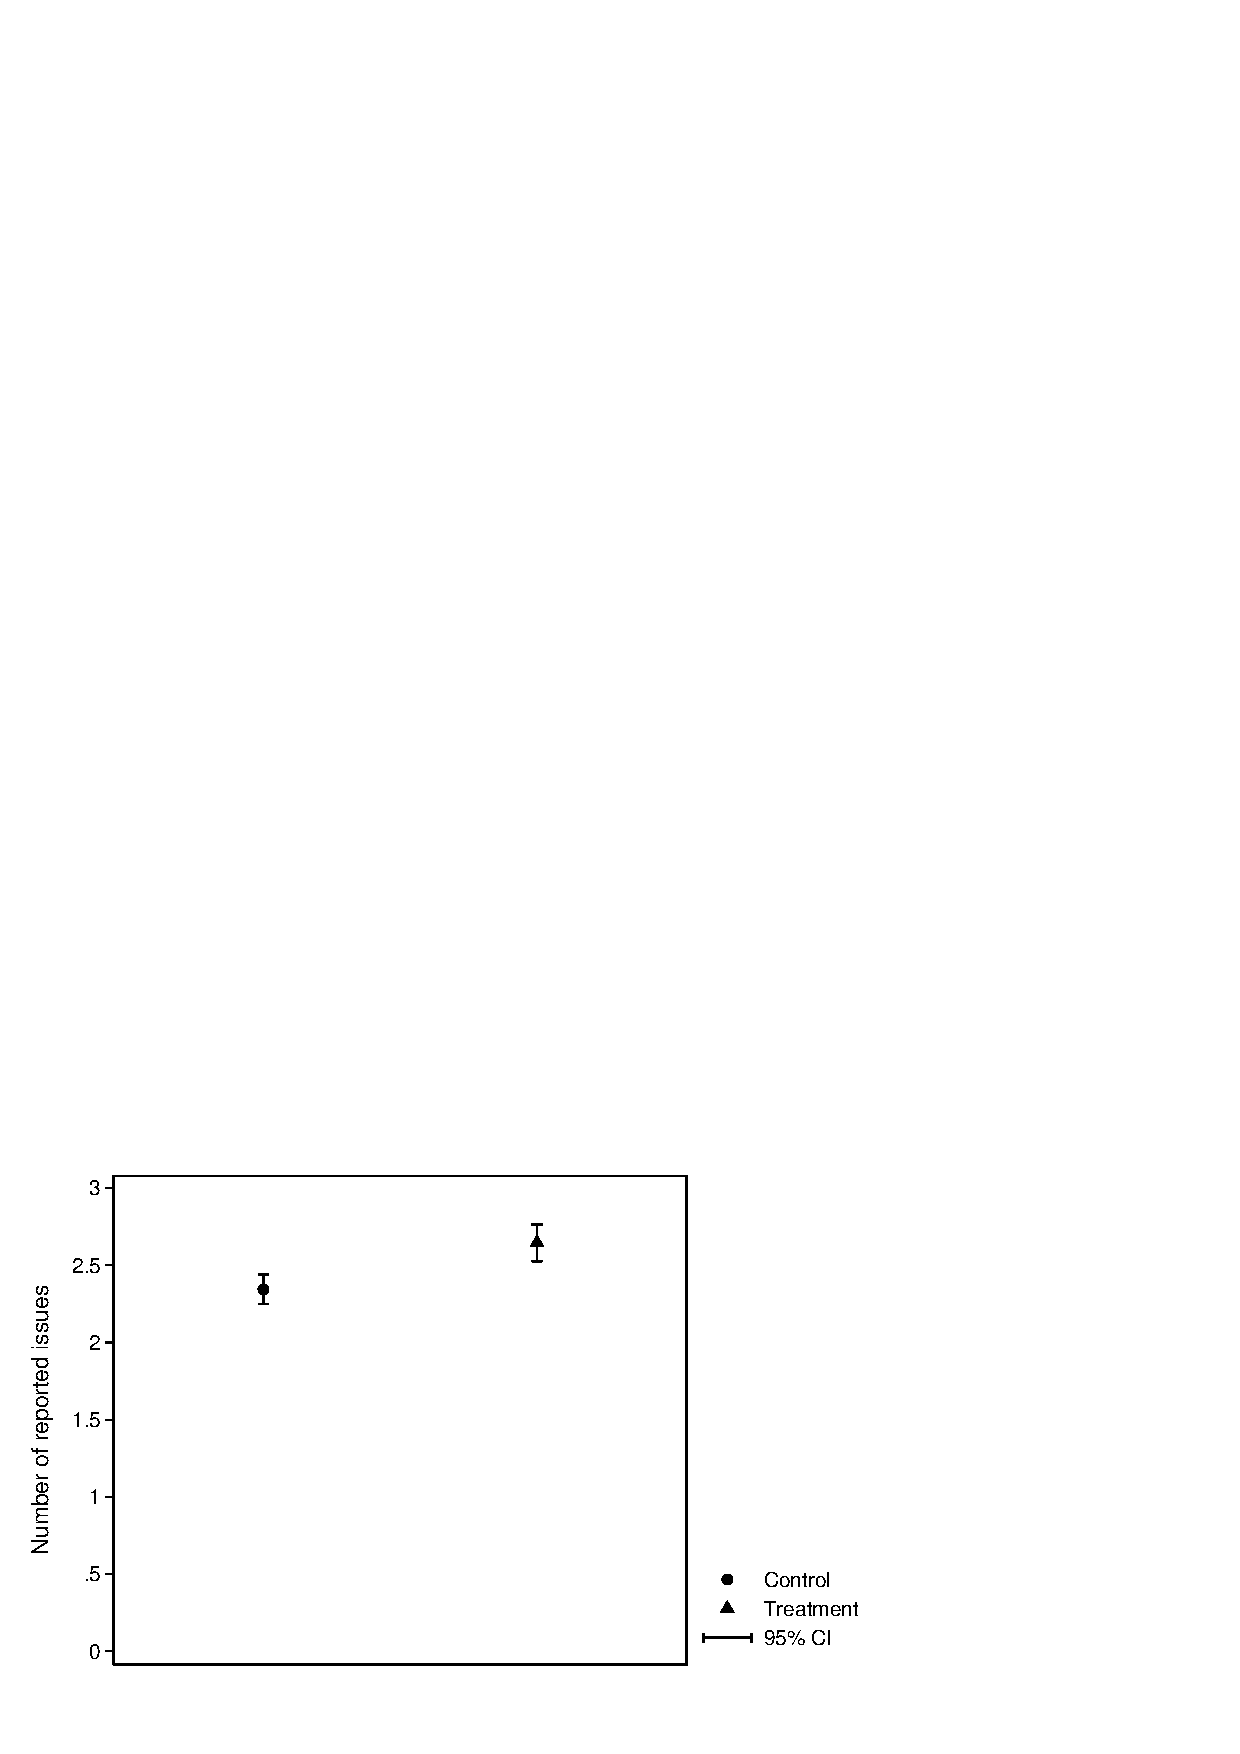
\includegraphics[width=0.6\linewidth]{\figureloc/meancompare_overall.png}
  \caption{Comparison of means of issues faced: treatment vs. control.}
  \label{fig:meancompare_overall}
\end{figure}

\subsection*{Conflict}
The first dimension over which I create sub-groups is conflict history. For this I combine two data sources:  I use data collected from an earlier round of the study that collected detailed conflict exposure data. This data was collected in 2012, and any relation between violent events and SGBV can't be due to direct victimization, whereby women are victimized by members of armed groups during these particular events. I then use more recent ACLED data, which is more likely to be indicative of direct effects.

First, I compare respondents who live in households that indicated in 2012 to have suffered loss of (or damage to) property, including agricultural fields, due to conflict. See top-left panel of \ref{fig:meancompare_conf}. In the non-victimized group (n=\incid{victimproplost0}{n}), the average number of issues was \incid{victimproplost0}{mean0} for the control group, and \incid{victimproplost0}{mean1} for the treatment group. This implies a rate of SGBV of \incid{victimproplost0}{incidence_pct}\% (p = \incid{victimproplost0}{p}). For the group that has suffered loss of property due to the conflict (n=\incid{victimproplost1}{n}), the average number of issues was \incid{victimproplost1}{mean0} for the control group, and \incid{victimproplost1}{mean1} for the treatment group. This implies a rate of SGBV of \incid{victimproplost1}{incidence_pct}\% (p = \incid{victimproplost1}{p}).

\begin{figure}[htb]
  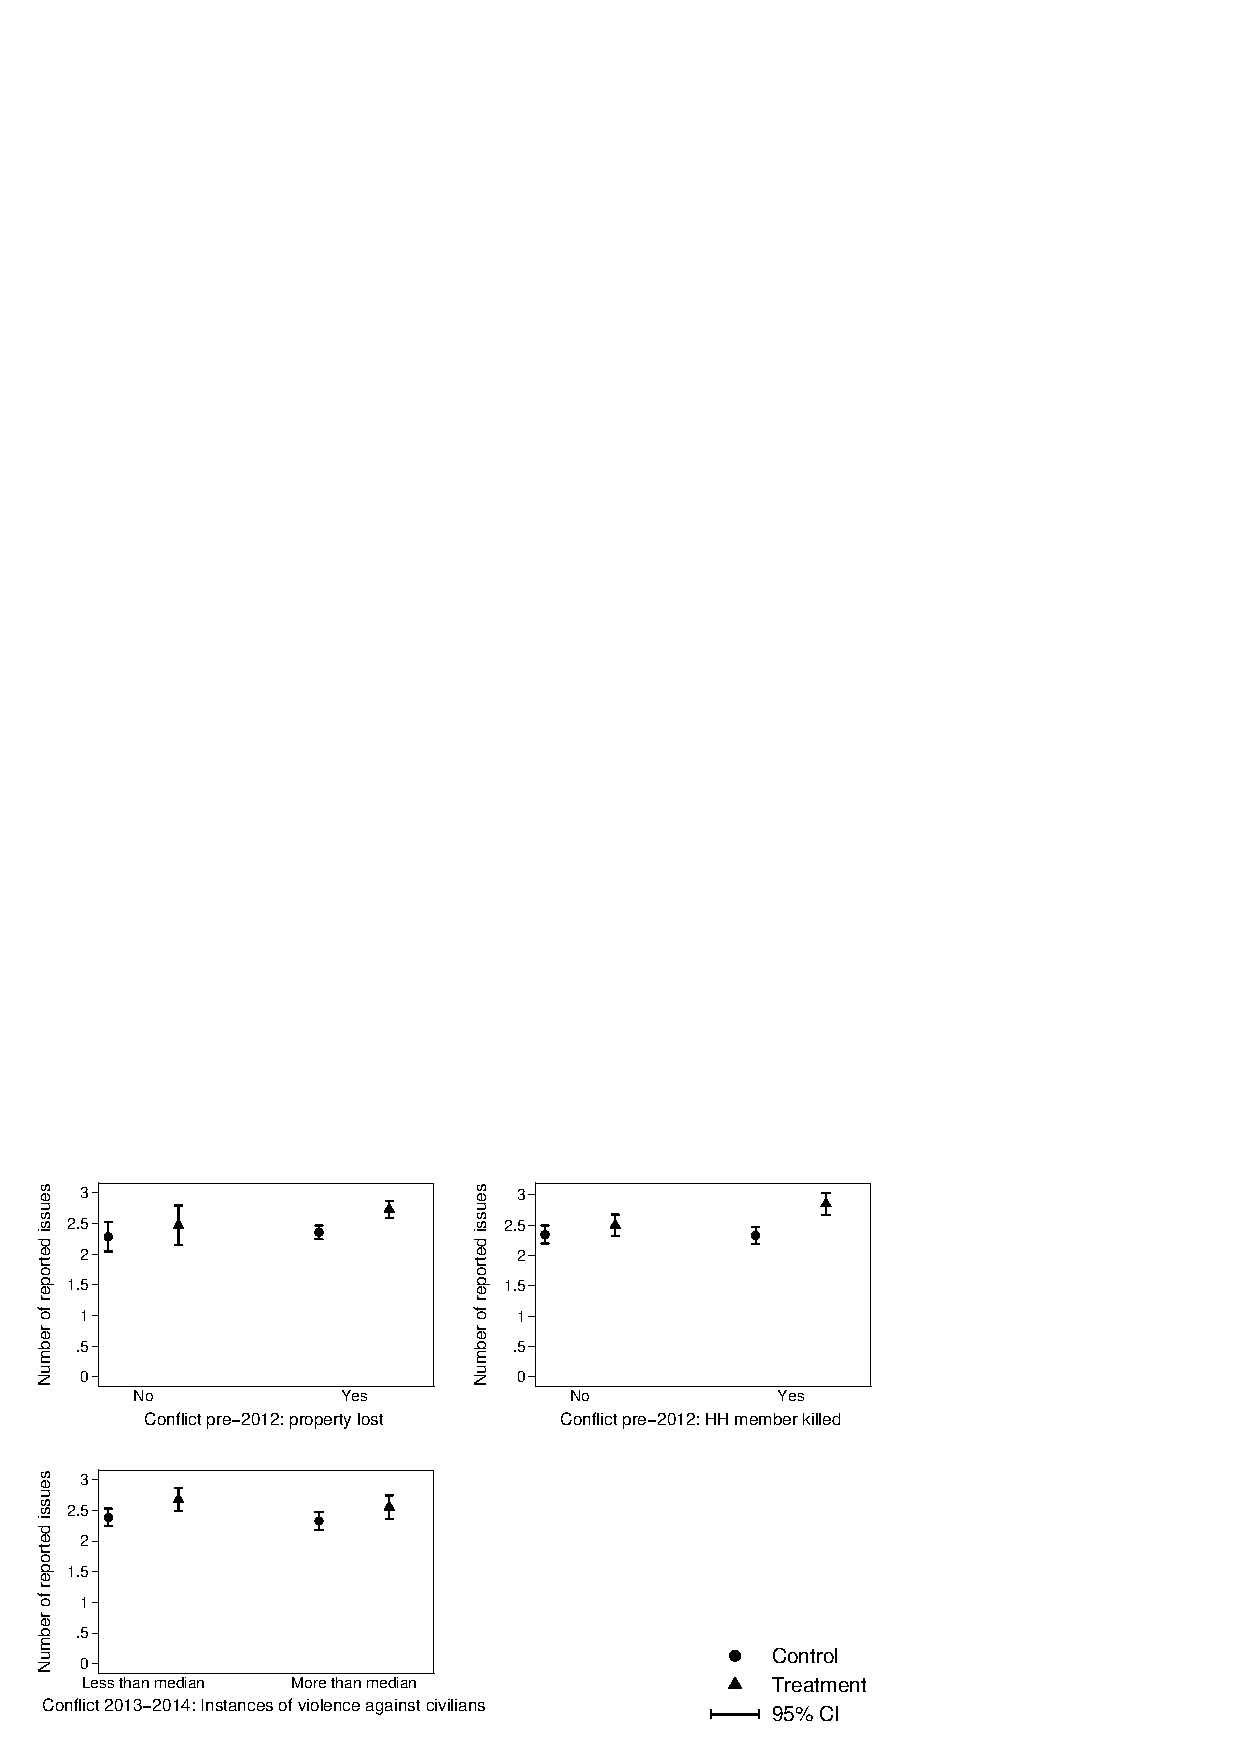
\includegraphics[width=\linewidth]{\figureloc/meancompare_conf.png}
  \caption{Comparison of means of issues faced across conflict exposure.}
  \label{fig:meancompare_conf}
\end{figure}

The second conflict indicator I examine, is whether the respondent's household indicated in 2012 to have lost any household members or family as a consequence of the conflict. See top-right panel of \ref{fig:meancompare_conf}. In the non-victimized group (n=\incid{victimfamlost0}{n}), the average number of issues was \incid{victimfamlost0}{mean0} for the control group, and \incid{victimfamlost0}{mean1} for the treatment group. This implies a rate of SGBV of \incid{victimfamlost0}{incidence_pct}\% (p = \incid{victimfamlost0}{p}). For the group that has suffered loss of property due to the conflict (n=\incid{victimfamlost1}{n}), the average number of issues was \incid{victimfamlost1}{mean0} for the control group, and \incid{victimfamlost1}{mean1} for the treatment group. This implies a rate of SGBV of \incid{victimfamlost1}{incidence_pct}\% (p = \incid{victimfamlost1}{p}).

The third conflict indicator I examine, is the number of cases of violence against civilians in ACLED data within a 10km radius during the past twelve months. Here, I split the sample in two, using the median as a cutoff point. See bottom-left panel of \ref{fig:meancompare_conf}. In the non-victimized group (n=\incid{acledviolence10d0}{n}), the average number of issues was \incid{acledviolence10d0}{mean0} for the control group, and \incid{acledviolence10d0}{mean1} for the treatment group. This implies a rate of SGBV of \incid{acledviolence10d0}{incidence_pct}\% (p = \incid{acledviolence10d0}{p}). For the group that has suffered loss of property due to the conflict (n=\incid{acledviolence10d1}{n}), the average number of issues was \incid{acledviolence30d1}{mean0} for the control group, and \incid{acledviolence10d1}{mean1} for the treatment group. This implies a rate of SGBV of \incid{acledviolence10d1}{incidence_pct}\% (p = \incid{acledviolence10d1}{p}). Note that the results presented here are robust to using number of battles or number of fatalities rather than the instances of violence against civilians; using 5,15,20, 25 or 30km as a radius, or using a continuous variable, rather than a binary variable.  

The average number of items reported by the groups created by the conflict indicators explored above is presented in Table \ref{tab:meandiff_conf}, for both treatment and control groups. The Diff columns thus provides the estimate of the incidence in each group. The difference in these differences is then presented in the Diff in Diff row for each variable. This estimate is equal to coefficient $\beta_3$ in equation \ref{eq:interaction} above. The only statistically significant Diff in Diff estimate is for having lost a household or family member due to conflict. Incidence for those woman without such loss is 21\%, for those with such loss it is 52\%. The difference of 31\% is significant a the 10\% level.

\begin{table}[htb]
\caption{Differences in numbers of issued faced in the list experiment, across conflict indicators}
\label{tab:meandiff_conf}
\meandifftab{"\tableloc/meandifftab_conf.csv"}
\end{table}

\subsection*{Intra-household bargaining position}
I then create sub-groups based on intra-household dynamics. First, I compare women across the relative status of the partners at the time of marriage. For this, I use the land held by the partners' families at the time of marriage as proxy for status (See top-left panel of Figure \ref{fig:meancompare_mar}). In the group where the wife had more status before the marriage (n=\incid{statpar1}{n}), the average number of issues was \incid{statpar1}{mean0} for the control group, and \incid{statpar1}{mean1} for the treatment group. The difference in means implies a rate of SGBV of \incid{statpar1}{incidence_pct}\% (p-value of a t-test on the means = \incid{statpar1}{p}). In the group where the partners were of equal standing (n=\incid{statpar2}{n}), the average number of issues was \incid{statpar2}{mean0} for the control group, and \incid{statpar2}{mean1} for the treatment group. This implies a rate of SGBV of \incid{statpar2}{incidence_pct} (p = \incid{statpar2}{p}). In the group where the husband had more status (n=\incid{statpar3}{n}), the average number of issues was \incid{statpar3}{mean0} for the control group, and \incid{statpar3}{mean1} for the treatment group. This implies a rate of SGBV of \incid{statpar3}{incidence_pct} (p = \incid{statpar3}{p}).

\begin{figure}[htb]
  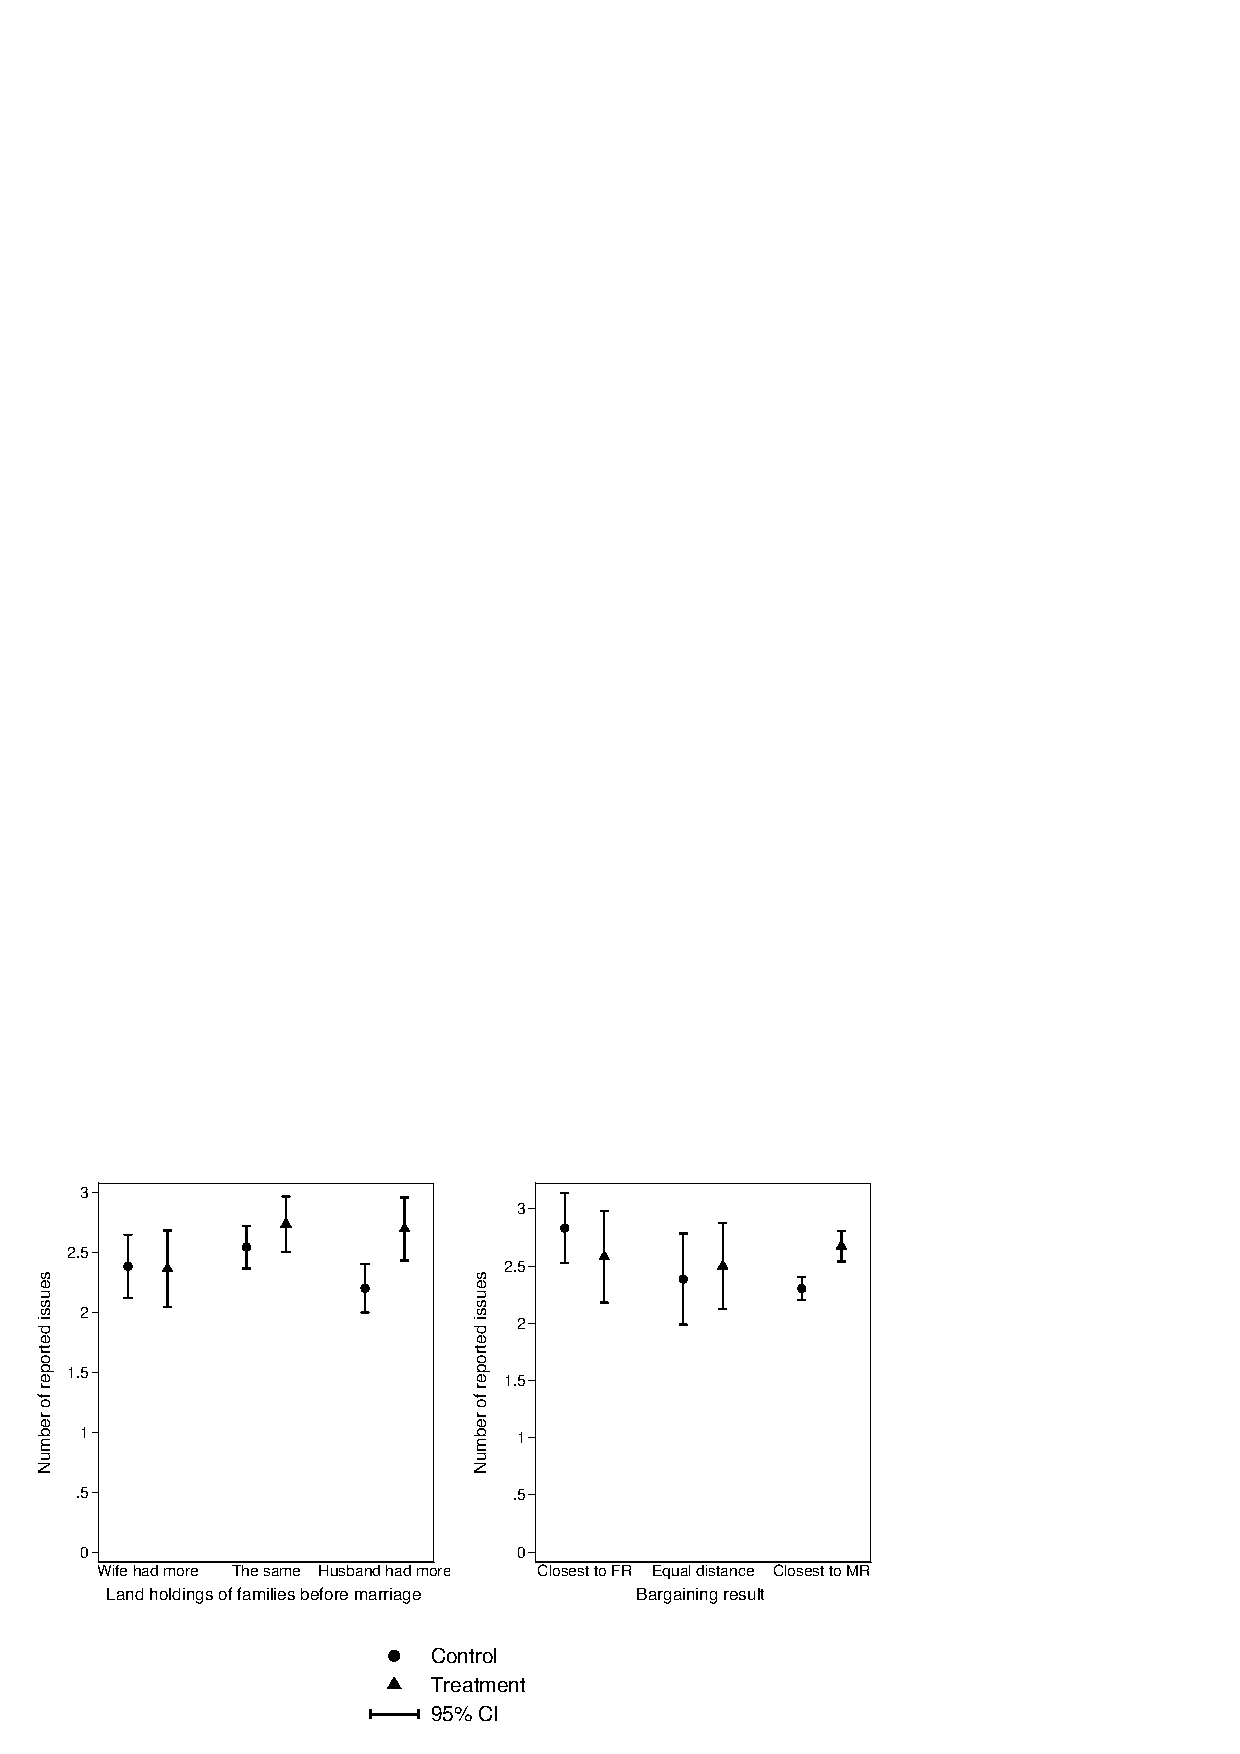
\includegraphics[width=\linewidth]{\figureloc/meancompare_mar.png}
  \caption{Comparison of means of issues faced by pre-marriage status.}
  \label{fig:meancompare_mar}
\end{figure}

The second intra-household aspect I explore is derived from the results of a bargaining game played with couples. Couples first took a decision individually, and then jointly. I then create three groups, based on whether the joint decision is closer to the husband's decision, to the wife's, or if the distance is equal. See top-right panel of figure \ref{fig:meancompare_mar}. In the group where the couple decision was closest to the wife's decision (n=\incid{bargresult1}{n}), the average number of issues was \incid{bargresult1}{mean0} for the control group, and \incid{bargresult1}{mean1} for the treatment group. This implies a rate of SGBV of \incid{bargresult1}{incidence_pct}\% (p = \incid{bargresult1}{p}). In the group where the couple decision was equally close to the husband and wife (n=\incid{bargresult2}{n}), the average number of issues was \incid{bargresult2}{mean0} for the control group, and \incid{bargresult2}{mean1} for the treatment group. This implies a rate of SGBV of \incid{bargresult2}{incidence_pct}\% (p = \incid{bargresult2}{p}). In the group where the couple decision was closest to the husband's (n=\incid{bargresult3}{n}), the average number of issues was \incid{bargresult3}{mean0} for the control group, and \incid{bargresult3}{mean1} for the treatment group. This implies a rate of SGBV of \incid{bargresult3}{incidence_pct}\% (p = \incid{bargresult3}{p}).

In Table \ref{tab:meadifftab_mar}, the estimates for incidence displayed graphically above are tabulated, including the diff in diff estimate for difference in incidence of SGBV between the groups created by each variable. In order for the interpretation of the Diff in Diff coefficient to remain the same across variables, the results for the bargaining game and the pre-marriage status were split into two indicator variables: one indicating the woman had more status (with households with equal status and where the husband had more status forming the reference group) and one indicating the husband had more status. The incidence of SGV for women whose husband's family owned more land than their own family is 33 percentage points higher than for other women. When looking at bargaining, women whose husband's choice in the game was closest to the joint decision faced incidence rates that were 57 percentage points higher than other women. Both these findings are significant at the 5\% level. 


\begin{table}[htb]
\caption{Differences in numbers of issued faced in the list experiment, across intra-household status}
\label{tab:meadifftab_mar}
\meandifftab{"C:/Users/Koen/Dropbox (Personal)/PhD/Papers/CongoGBV/Tables/meandifftab_mar.csv"}
\end{table}

\subsection*{Gender Attitudes}
I then explore the relationship between gender attitudes of both partners, and the incidence of SGBV. The first indicator I consider, is the attitudes of the husband (left-hand panel of Figure \ref{fig:meancompare_att}. For this, I recode the answers so that 5 is always fully agree with the empowered proposition, and 1 is fully agree with the less empowered option. I then sum all the answers, and for easy interpretation split the sample by the median answer. In the group where husband's attitudes are less empowered than the median (n=\incid{atthusbtotalbin0}{n}), the average number of issues was \incid{atthusbtotalbin0}{mean0} for the control group, and \incid{atthusbtotalbin0}{mean1} for the treatment group. This implies a rate of SGBV of \incid{atthusbtotalbin0}{incidence_pct}\% (p = \incid{atthusbtotalbin0}{p}). For the group with husband that are more empowered than the median (n=\incid{atthusbtotalbin1}{n}), the average number of issues was \incid{atthusbtotalbin1}{mean0} for the control group, and \incid{atthusbtotalbin1}{mean1} for the treatment group. This implies a rate of SGBV of \incid{atthusbtotalbin1}{incidence_pct}\% (p = \incid{atthusbtotalbin1}{p}).

\begin{figure}[htb]
  \includegraphics[width=\linewidth]{\figureloc/meancompare_att.png}
  \caption{Comparison of means of issues faced across Husband's gender attitudes.}
  \label{fig:meancompare_att}
\end{figure}

The second indicator I consider, is the attitudes of the wife, using the same methods to split the sample as above (right-hand panel of Figure \ref{fig:meancompare_att}). In the group where wife's attitudes are less empowered than the median (n=\incid{attwifetotalbin0}{n}), the average number of issues was \incid{attwifetotalbin0}{mean0} for the control group, and \incid{attwifetotalbin0}{mean1} for the treatment group. This implies a rate of SGBV of \incid{attwifetotalbin0}{incidence_pct}\% (p = \incid{attwifetotalbin0}{p}). For the group with husband that are more empowered than the median (n=\incid{attwifetotalbin1}{n}), the average number of issues was \incid{attwifetotalbin1}{mean0} for the control group, and \incid{attwifetotalbin1}{mean1} for the treatment group. This implies a rate of SGBV of \incid{attwifetotalbin1}{incidence_pct}\% (p = \incid{attwifetotalbin1}{p}).

In Table \ref{tab:meadifftab_att}, the estimates for incidence that were displayed graphically above are tabulated, including the diff in diff estimate for difference in incidence of SGBV between the groups created by each variable. Of note is the large negative coefficient for the diff-in-diff on male empowerment attitudes. However, this coefficient is not statistically significant, possibly due to the relatively small number of men interviewed (see Table \ref{tab:bargsample}). The diff-in-diff estimate for female empowerment attitudes is smaller, and also not statistically significant.


\begin{table}[htb]
\caption{Differences in numbers of issued faced in the list experiment, across Gender Attitudes}
\label{tab:meadifftab_att}
\meandifftab{"C:/Users/Koen/Dropbox (Personal)/PhD/Papers/CongoGBV/Tables/meandifftab_att.csv"}
\end{table}


\subsection*{Multivariate Regression analysis}
\newcommand{\coeffget}[3]{\csvreader[filter=\equal{\reg}{#1} \and \equal{\var}{#2}]{\tableloc/regs.csv}{var=\var,reg=\reg,#3=\coeff}{\coeff}}

In the preceding sections, I examined univariate relations between variables of interest and the incidence of SGBV. However, such analysis may suffer from missing variables and spurious correlations. Here I move to a richer specification, in order to assess the relative impact of each variable. I expand equation \ref{eq:interaction} to include indicators for conflict, intra-household bargaining position and empowerment. To reduce the risk of multi-collinearity, I do not include the full set of variables discussed above, but select one indicator for each, guided by the results obtained above. A key criterion for selection is the number of respondents for each indicator. The analysis of list experiments suffers from rapid loss of power due to the indirect nature of the analysis. To mitigate this, indicators that are available for large groups of respondents were selected. For conflict, I include both the indicator for household member killed before 2012 (as an indicator for historic conflict) and violence against civilians from the ACLED data (as an indicator for recent conflict); for intra-household bargaining position a dummy for the husband's family having the most land; and for household bargaining, I use the attitudes of the wife. For these regression, I use the KICT Stata package developed by \citet{Tsai2019}; interpretation of the coefficients is the same as equation \ref{eq:interaction}, but estimation is more efficient.

In order to reduce missing variable bias, I include a set of controls that likely (co-)determine SGBV and the right-hand side variables listed above. A full analysis of these determinants is provided in the Appendix, Table \ref{tab:determinants_regression}. In particular, I include an indicator for the Female Respondent having a secondary education, the household owning livestock, and territory dummies. As seen in Table \ref{tab:conflict_by_terr} above, conflict experience differs across the territories in the study. 

In Table \ref{tab:results_regression} I display the results of these regressions. In columns 1-3 I rerun the univariate models from above. Results are the same as before: both conflict history and intra-household bargaining are associated with increased incidence of SGBV. I In column 4 I present the full model. I find that women in a marriage where their husband's family had more land before the marriage, are \coeffget{l5}{Delta:husbmoreland}{coef_pct} percentage points more likely than other women to be victim of SGBV. Women who live in households that lost a family or household member due to conflict prior to 2012 are \coeffget{l5}{Delta:victimfamlost}{coef_pct} percentage points more likely to be victimized by SGBV than other women. I find no statistically significant relation between empowerment norms, and SGBV or recent conflict and SGBV victimization.

The finding that conflict history is associated with an increase in SGBV, while recent conflict is not, points to the indirect relationship between conflict and SGBV, where conflict may affect SGBV rates not through perpetration by armed groups, but by an increase in IPV.

\begin{threeparttable}
	\caption{Multivariate regression Results}\label{tab:results_regression}
	\begin{center}
	{
\def\sym#1{\ifmmode^{#1}\else\(^{#1}\)\fi}
\begin{tabular}{l*{4}{c}}
\hline\hline
                    &\multicolumn{1}{c}{(1)}   &\multicolumn{1}{c}{(2)}   &\multicolumn{1}{c}{(3)}   &\multicolumn{1}{c}{(4)}   \\
\hline
Family MR had more land&       0.419** &               &               &       0.451*  \\
                    &     (0.204)   &               &               &     (0.240)   \\
[1em]
Conflict pre-2012: HH member killed&               &       0.409** &               &       0.374** \\
                    &               &     (0.182)   &               &     (0.179)   \\
[1em]
Conflict 2013-2014: Viol. against civilians&               &               &      0.0120   &      0.0147   \\
                    &               &               &    (0.0224)   &    (0.0230)   \\
[1em]
FR empowerment attitudes&               &               &               &    0.000101   \\
                    &               &               &               &    (0.0199)   \\
[1em]
Age of FR           &     0.00843   &     0.00684   &     0.00563   &      0.0110   \\
                    &    (0.0161)   &    (0.0182)   &    (0.0186)   &    (0.0207)   \\
[1em]
Age of MR           &     -0.0122   &    -0.00929   &    -0.00778   &     -0.0111   \\
                    &    (0.0149)   &    (0.0162)   &    (0.0174)   &    (0.0189)   \\
[1em]
HH Head Female      &     0.00951   &     -0.0766   &       0.257   &       0.421   \\
                    &     (0.445)   &     (0.525)   &     (0.318)   &     (0.410)   \\
[1em]
FR completed secondary education&      -1.111***&      -1.347***&      -1.034***&      -1.249***\\
                    &     (0.320)   &     (0.351)   &     (0.336)   &     (0.332)   \\
[1em]
MR completed primary education&     -0.0390   &     -0.0655   &      -0.193   &      -0.263   \\
                    &     (0.166)   &     (0.178)   &     (0.181)   &     (0.177)   \\
[1em]
Household has a tin roof&       0.292   &       0.279   &       0.184   &       0.214   \\
                    &     (0.203)   &     (0.221)   &     (0.234)   &     (0.233)   \\
[1em]
Household owns livestock&     -0.0455   &    -0.00342   &      -0.142   &      -0.193   \\
                    &     (0.160)   &     (0.181)   &     (0.177)   &     (0.186)   \\
[1em]
territory==Uvira    &       0.418   &       0.202   &       0.438   &       0.205   \\
                    &     (0.264)   &     (0.342)   &     (0.288)   &     (0.360)   \\
[1em]
territory==Fizi     &       0.511*  &       0.232   &       0.504*  &       0.191   \\
                    &     (0.292)   &     (0.365)   &     (0.302)   &     (0.379)   \\
[1em]
Project Beneficary  &      0.0542   &      0.0121   &      0.0382   &      0.0732   \\
                    &     (0.163)   &     (0.177)   &     (0.157)   &     (0.167)   \\
[1em]
Constant            &      -0.162   &    -0.00267   &    -0.00290   &      -0.111   \\
                    &     (0.483)   &     (0.506)   &     (0.491)   &     (0.614)   \\
\hline
Observations        &         449   &         402   &         379   &         350   \\
\hline\hline
\end{tabular}
}

	
	\begin{tablenotes}
	\small
	 \item Standard errors clustered at the village level
	 \item * p $<$ 0.1, **, p $<$ 0.05, *** p $<$ 0.01
	\end{tablenotes}
	\end{center}
\end{threeparttable}

\section*{Conclusion}
%restate the topic and its importance.
This study provided evidence on the victims of SGBV in Congo. Prevalence of SGBV is high in Congo, but little is known about the victims. To obtain this evidence, I used a list experiment to prevent disclosure bias.This allows me to find correlates of SGBV. I complemented this with a household bargaining game, designed to elicit often unobserved intra-household dynamics.

The incidence rates I find are very high: 30\% of the women in the sample report having been the victim of SGBV \textit{in the past twelve months}. This high rate is not likely to be nationally, or regionally, representative. The women in the sample were recruited among beneficiaries and potential beneficiaries of programs aimed at assisting the most vulnerable women and households. It is to be expected that incidence rates in this group are higher than for other groups.

When examining the backgrounds of the victims, I find that they are likely to be married to higher-status men, have low bargaining power, and have been exposed to violent conflict to the extent where they have lost family or household members. When comparing these two effects in one analysis, I find that the effect of intra-household dynamics is larger than the effect of conflict. This contrasts with popular frames where the conflict is seen as the primary driver of SGBV, but is in line with previous literature suggesting that intimate partners are more likely perpetrators of SGBV than members of armed groups \citep[see e.g.][]{Peterman2011}. 

While I find some evidence that victims of violence have less empowered attitudes than other women, this effect is small. This suggests that the focus of interventions aiming to reduce SGBV should be on the attitudes of women, but on their bargaining position in the household.

There are two large caveats with these findings: (i) they are not causal; (ii) little analysis could be done on the perpetrators of the violence, as indirect questioning precludes probing into this. More research is needed to  to address these important issues.

%bibliography, this is needed for bibtex
\clearpage 
\bibliographystyle{chicago}
%path to .bib file (e.g. automatically exported by mendeley) dot not include the file extension!
\bibliography{C:/Users/Koen/Dropbox/Literatuur/Mendeley/Bibtex/CongoGBV}

\clearpage
\section*{Appendix}
\setcounter{table}{0}
\renewcommand{\thetable}{A\arabic{table}}

\begin{threeparttable}[htb]
	\caption{Sample selection for the Gender Module}\label{tab:sample_selection}
	\begin{center}
	{
\def\sym#1{\ifmmode^{#1}\else\(^{#1}\)\fi}
\begin{tabular}{l*{3}{c}}
\hline\hline
                    &\multicolumn{1}{c}{(1)}   &\multicolumn{1}{c}{(2)}   &\multicolumn{1}{c}{(3)}   \\
                    &        Wife   &     Husband   &      Couple   \\
\hline
                    &               &               &               \\
Age of FR           &     -0.0305** &      0.0244** &     -0.0124   \\
                    &    (0.0126)   &    (0.0112)   &    (0.0127)   \\
[1em]
Age of MR           &      0.0199*  &    -0.00864   &      0.0176   \\
                    &    (0.0118)   &    (0.0110)   &    (0.0130)   \\
[1em]
HH Head Female      &       0.171   &      -1.142*  &            \\
                    &     (0.689)   &     (0.602)   &            \\
[1em]
FR completed primary education&       0.120   &      -0.197   &      -0.109   \\
                    &     (0.224)   &     (0.245)   &     (0.210)   \\
[1em]
FR completed secondary education&       0.484   &      -0.285   &       0.169   \\
                    &     (0.587)   &     (0.399)   &     (0.488)   \\
[1em]
MR completed primary education&     -0.0233   &       0.226   &       0.279   \\
                    &     (0.189)   &     (0.218)   &     (0.230)   \\
[1em]
MR completed secondary education&       0.228   &      -0.208   &    -0.00740   \\
                    &     (0.213)   &     (0.215)   &     (0.212)   \\
[1em]
Household has a tin roof&       0.307*  &      0.0468   &       0.446** \\
                    &     (0.181)   &     (0.171)   &     (0.207)   \\
[1em]
Household owns livestock&      -0.564***&       0.695***&       0.146   \\
                    &     (0.204)   &     (0.189)   &     (0.172)   \\
[1em]
territory==Uvira    &      -0.215   &       1.165***&       0.949***\\
                    &     (0.297)   &     (0.261)   &     (0.336)   \\
[1em]
territory==Fizi     &     -0.0496   &       0.312   &       0.258   \\
                    &     (0.263)   &     (0.217)   &     (0.296)   \\
[1em]
Project Beneficary  &       0.490** &      -0.450** &      0.0594   \\
                    &     (0.195)   &     (0.182)   &     (0.249)   \\
[1em]
Constant            &       0.726*  &      -0.700   &      -2.347***\\
                    &     (0.430)   &     (0.434)   &     (0.429)   \\
\hline
Observations        &         717   &         717   &         704   \\
\hline\hline
\end{tabular}
}

	\begin{tablenotes}
	\small
	 \item Standard errors clustered at the village level
	 \item * p $<$ 0.1, **, p $<$ 0.05, *** p $<$ 0.01
	\end{tablenotes}
	\end{center}
\end{threeparttable}

\begin{landscape}


\begin{threeparttable}
	\caption{Determinants of Violence, Bargaining Power and Empowerment Norms}\label{tab:determinants_regression}
	\tiny
	\centering
	{
\def\sym#1{\ifmmode^{#1}\else\(^{#1}\)\fi}
\begin{tabular}{l*{3}{c}}
\hline\hline
                    &\multicolumn{1}{c}{(1)}&\multicolumn{1}{c}{(2)}&\multicolumn{1}{c}{(3)}\\
                    &\multicolumn{1}{c}{\specialcell{Family MR\\had more land}}&\multicolumn{1}{c}{\specialcell{Bargaining:\\closer to FR}}&\multicolumn{1}{c}{\specialcell{Conflict pre-2012:\\HH member killed}}\\
\hline
Family MR had more land&               &      0.0756   &       0.679   \\
                    &               &    (0.0554)   &     (0.476)   \\
[1em]
Conflict pre-2012: HH member killed&      0.0799   &               &      -1.494***\\
                    &    (0.0588)   &               &     (0.476)   \\
[1em]
Conflict 2013-2014: Viol. against civilians&     0.00885   &     -0.0184***&               \\
                    &   (0.00627)   &   (0.00477)   &               \\
[1em]
Age of FR           &    -0.00431   &     0.00219   &     -0.0264   \\
                    &   (0.00602)   &   (0.00448)   &    (0.0349)   \\
[1em]
Age of MR           &     0.00355   &    -0.00146   &      0.0281   \\
                    &   (0.00435)   &   (0.00390)   &    (0.0320)   \\
[1em]
FR completed primary education&      0.0542   &      -0.109   &     -0.0536   \\
                    &    (0.0695)   &    (0.0656)   &     (0.672)   \\
[1em]
FR completed secondary education&     -0.0147   &       0.474***&       0.602   \\
                    &     (0.129)   &     (0.147)   &     (1.417)   \\
[1em]
MR completed primary education&      0.0834   &      0.0314   &      -0.347   \\
                    &    (0.0612)   &    (0.0622)   &     (0.512)   \\
[1em]
MR completed secondary education&     -0.0523   &      0.0408   &       0.239   \\
                    &    (0.0703)   &    (0.0764)   &     (0.603)   \\
[1em]
Household has a tin roof&     -0.0267   &      -0.114** &       0.563   \\
                    &    (0.0537)   &    (0.0509)   &     (0.539)   \\
[1em]
Household owns livestock&       0.114** &      0.0536   &      -0.235   \\
                    &    (0.0554)   &    (0.0526)   &     (0.490)   \\
[1em]
territory==Uvira    &     -0.0556   &       0.295***&       3.566***\\
                    &    (0.0589)   &    (0.0904)   &     (1.104)   \\
[1em]
territory==Fizi     &     -0.0166   &       0.404***&      -1.069   \\
                    &    (0.0560)   &    (0.0763)   &     (1.487)   \\
[1em]
Project Beneficary  &     -0.0854*  &      0.0492   &       0.198   \\
                    &    (0.0461)   &    (0.0450)   &     (1.136)   \\
[1em]
Constant            &       0.212   &       0.247** &       6.599***\\
                    &     (0.133)   &     (0.106)   &     (1.420)   \\
\hline
Observations        &         350   &         350   &         350   \\
\hline\hline
\end{tabular}
}

	
	\begin{tablenotes}
	\tiny
	 \item Standard errors clustered at the village level
	 \item * p $<$ 0.1, **, p $<$ 0.05, *** p $<$ 0.01
	\end{tablenotes}
\end{threeparttable}
\end{landscape}
\end{document}
